% Created 2017-02-01 Wed 04:43
% Intended LaTeX compiler: pdflatex
\documentclass[11pt]{article}
\usepackage[utf8]{inputenc}
\usepackage[T1]{fontenc}
\usepackage{graphicx}
\usepackage{grffile}
\usepackage{longtable}
\usepackage{wrapfig}
\usepackage{rotating}
\usepackage[normalem]{ulem}
\usepackage{amsmath}
\usepackage{textcomp}
\usepackage{amssymb}
\usepackage{capt-of}
\usepackage{hyperref}
\author{Jake Brawer}
\date{\today}
\title{HW 1\\\medskip
\large CPSC424}
\hypersetup{
 pdfauthor={Jake Brawer},
 pdftitle={HW 1},
 pdfkeywords={},
 pdfsubject={},
 pdfcreator={Emacs 25.1.1 (Org mode 9.0.3)}, 
 pdflang={English}}
\begin{document}

\maketitle

\section{Building and Running the Code}
\label{sec:orgd3dac10}

\subsection{Software and Dev. Environments}
\label{sec:org6d1c1e5}

All the programming for this assignment was done in vim. This document, including the figures, were made using emacs (and gnuplot). The only module loaded used in this assignment is Langs/Intel/15.

\subsection{Env Output}
\label{sec:org79706c2}
MKLROOT=/home/apps/fas/Langs/Intel/2015\(_{\text{update2}}\)/composer\(_{\text{xe}}\)\(_{\text{2015.2.164}}\)/mkl
MANPATH=/home/apps/fas/Langs/Intel/2015\(_{\text{update2}}\)/composer\(_{\text{xe}}\)\(_{\text{2015.2.164}}\)/man/en\(_{\text{US}}\):/home/apps/fas/Langs/Intel/2015\(_{\text{update2}}\)/composer\(_{\text{xe}}\)\(_{\text{2015.2.164}}\)/debugger/gdb/intel64/share/man/:/home/apps/fas/Langs/Intel/2015\(_{\text{update2}}\)/composer\(_{\text{xe}}\)\(_{\text{2015.2.164}}\)/debugger/gdb/intel64\(_{\text{mic}}\)/share/man/:/usr/share/man:/opt/moab/share/man:
GDB\(_{\text{HOST}}\)=/home/apps/fas/Langs/Intel/2015\(_{\text{update2}}\)/composer\(_{\text{xe}}\)\(_{\text{2015.2.164}}\)/debugger/gdb/intel64\(_{\text{mic}}\)/bin/gdb-ia-mic
HOSTNAME=login-0-0.local
IPPROOT=/home/apps/fas/Langs/Intel/2015\(_{\text{update2}}\)/composer\(_{\text{xe}}\)\(_{\text{2015.2.164}}\)/ipp
INTEL\(_{\text{LICENSE}}\)\(_{\text{FILE}}\)=/home/apps/fas/Langs/Intel/2015\(_{\text{update2}}\)/composer\(_{\text{xe}}\)\(_{\text{2015.2.164}}\)/licenses:/opt/intel/licenses:/home/apps/fas/Licenses/intel\(_{\text{site.lic}}\)
TERM=xterm
SHELL=/bin/bash
HISTSIZE=1000
GDBSERVER\(_{\text{MIC}}\)=/home/apps/fas/Langs/Intel/2015\(_{\text{update2}}\)/composer\(_{\text{xe}}\)\(_{\text{2015.2.164}}\)/debugger/gdb/target/mic/bin/gdbserver
SSH\(_{\text{CLIENT}}\)=172.27.41.66 41162 22
LIBRARY\(_{\text{PATH}}\)=/home/apps/fas/Langs/Intel/2015\(_{\text{update2}}\)/composer\(_{\text{xe}}\)\(_{\text{2015.2.164}}\)/ipp/../compiler/lib/intel64:/home/apps/fas/Langs/Intel/2015\(_{\text{update2}}\)/composer\(_{\text{xe}}\)\(_{\text{2015.2.164}}\)/ipp/lib/intel64:/home/apps/fas/Langs/Intel/2015\(_{\text{update2}}\)/composer\(_{\text{xe}}\)\(_{\text{2015.2.164}}\)/compiler/lib/intel64:/home/apps/fas/Langs/Intel/2015\(_{\text{update2}}\)/composer\(_{\text{xe}}\)\(_{\text{2015.2.164}}\)/mkl/lib/intel64:/home/apps/fas/Langs/Intel/2015\(_{\text{update2}}\)/composer\(_{\text{xe}}\)\(_{\text{2015.2.164}}\)/tbb/lib/intel64/gcc4.4
PERL5LIB=/opt/moab/lib/perl5
FPATH=/home/apps/fas/Langs/Intel/2015\(_{\text{update2}}\)/composer\(_{\text{xe}}\)\(_{\text{2015.2.164}}\)/mkl/include
QTDIR=/usr/lib64/qt-3.3
QTINC=/usr/lib64/qt-3.3/include
MIC\(_{\text{LD}}\)\(_{\text{LIBRARY}}\)\(_{\text{PATH}}\)=/home/apps/fas/Langs/Intel/2015\(_{\text{update2}}\)/composer\(_{\text{xe}}\)\(_{\text{2015.2.164}}\)/mpirt/lib/mic:/home/apps/fas/Langs/Intel/2015\(_{\text{update2}}\)/composer\(_{\text{xe}}\)\(_{\text{2015.2.164}}\)/ipp/lib/mic:/home/apps/fas/Langs/Intel/2015\(_{\text{update2}}\)/composer\(_{\text{xe}}\)\(_{\text{2015.2.164}}\)/compiler/lib/mic:/home/apps/fas/Langs/Intel/2015\(_{\text{update2}}\)/composer\(_{\text{xe}}\)\(_{\text{2015.2.164}}\)/mkl/lib/mic:/opt/intel/mic/coi/device-linux-release/lib:/opt/intel/mic/myo/lib:/home/apps/fas/Langs/Intel/2015\(_{\text{update2}}\)/composer\(_{\text{xe}}\)\(_{\text{2015.2.164}}\)/tbb/lib/mic
SSH\(_{\text{TTY}}\)=/dev/pts/63
ANT\(_{\text{HOME}}\)=/opt/rocks
USER=jnb37
LD\(_{\text{LIBRARY}}\)\(_{\text{PATH}}\)=/home/apps/fas/Langs/Intel/2015\(_{\text{update2}}\)/composer\(_{\text{xe}}\)\(_{\text{2015.2.164}}\)/mpirt/lib/intel64:/home/apps/fas/Langs/Intel/2015\(_{\text{update2}}\)/composer\(_{\text{xe}}\)\(_{\text{2015.2.164}}\)/ipp/../compiler/lib/intel64:/home/apps/fas/Langs/Intel/2015\(_{\text{update2}}\)/composer\(_{\text{xe}}\)\(_{\text{2015.2.164}}\)/ipp/lib/intel64:/home/apps/fas/Langs/Intel/2015\(_{\text{update2}}\)/composer\(_{\text{xe}}\)\(_{\text{2015.2.164}}\)/ipp/tools/intel64/perfsys:/opt/intel/mic/coi/host-linux-release/lib:/opt/intel/mic/myo/lib:/home/apps/fas/Langs/Intel/2015\(_{\text{update2}}\)/composer\(_{\text{xe}}\)\(_{\text{2015.2.164}}\)/compiler/lib/intel64:/home/apps/fas/Langs/Intel/2015\(_{\text{update2}}\)/composer\(_{\text{xe}}\)\(_{\text{2015.2.164}}\)/mkl/lib/intel64:/home/apps/fas/Langs/Intel/2015\(_{\text{update2}}\)/composer\(_{\text{xe}}\)\(_{\text{2015.2.164}}\)/tbb/lib/intel64/gcc4.4:/home/apps/fas/Langs/Intel/2015\(_{\text{update2}}\)/composer\(_{\text{xe}}\)\(_{\text{2015.2.164}}\)/debugger/ipt/intel64/lib
MIC\(_{\text{LIBRARY}}\)\(_{\text{PATH}}\)=/home/apps/fas/Langs/Intel/2015\(_{\text{update2}}\)/composer\(_{\text{xe}}\)\(_{\text{2015.2.164}}\)/compiler/lib/mic:/home/apps/fas/Langs/Intel/2015\(_{\text{update2}}\)/composer\(_{\text{xe}}\)\(_{\text{2015.2.164}}\)/mpirt/lib/mic:/home/apps/fas/Langs/Intel/2015\(_{\text{update2}}\)/composer\(_{\text{xe}}\)\(_{\text{2015.2.164}}\)/tbb/lib/mic
ROCKS\(_{\text{ROOT}}\)=/opt/rocks
CPATH=/home/apps/fas/Langs/Intel/2015\(_{\text{update2}}\)/composer\(_{\text{xe}}\)\(_{\text{2015.2.164}}\)/ipp/include:/home/apps/fas/Langs/Intel/2015\(_{\text{update2}}\)/composer\(_{\text{xe}}\)\(_{\text{2015.2.164}}\)/mkl/include:/home/apps/fas/Langs/Intel/2015\(_{\text{update2}}\)/composer\(_{\text{xe}}\)\(_{\text{2015.2.164}}\)/tbb/include
YHPC\(_{\text{COMPILER}}\)=Intel
NLSPATH=/home/apps/fas/Langs/Intel/2015\(_{\text{update2}}\)/composer\(_{\text{xe}}\)\(_{\text{2015.2.164}}\)/compiler/lib/intel64/locale/\%l\_\%t/\%N:/home/apps/fas/Langs/Intel/2015\(_{\text{update2}}\)/composer\(_{\text{xe}}\)\(_{\text{2015.2.164}}\)/ipp/lib/intel64/locale/\%l\_\%t/\%N:/home/apps/fas/Langs/Intel/2015\(_{\text{update2}}\)/composer\(_{\text{xe}}\)\(_{\text{2015.2.164}}\)/mkl/lib/intel64/locale/\%l\_\%t/\%N:/home/apps/fas/Langs/Intel/2015\(_{\text{update2}}\)/composer\(_{\text{xe}}\)\(_{\text{2015.2.164}}\)/debugger/gdb/intel64\(_{\text{mic}}\)/share/locale/\%l\_\%t/\%N:/home/apps/fas/Langs/Intel/2015\(_{\text{update2}}\)/composer\(_{\text{xe}}\)\(_{\text{2015.2.164}}\)/debugger/gdb/intel64/share/locale/\%l\_\%t/\%N
MAIL=/var/spool/mail/jnb37
PATH=/home/apps/fas/Langs/Intel/2015\(_{\text{update2}}\)/composer\(_{\text{xe}}\)\(_{\text{2015.2.164}}\)/bin/intel64:/home/apps/fas/Langs/Intel/2015\(_{\text{update2}}\)/composer\(_{\text{xe}}\)\(_{\text{2015.2.164}}\)/mpirt/bin/intel64:/home/apps/fas/Langs/Intel/2015\(_{\text{update2}}\)/composer\(_{\text{xe}}\)\(_{\text{2015.2.164}}\)/debugger/gdb/intel64\(_{\text{mic}}\)/bin:/home/apps/fas/Langs/Intel/2015\(_{\text{update2}}\)/composer\(_{\text{xe}}\)\(_{\text{2015.2.164}}\)/debugger/gdb/intel64/bin:/home/apps/fas/Modules:/usr/lib64/qt-3.3/bin:/opt/moab/bin:/usr/local/bin:/bin:/usr/bin:/usr/local/sbin:/usr/sbin:/sbin:/usr/java/latest/bin:/opt/rocks/bin:/opt/rocks/sbin:/home/apps/bin:/home/fas/cpsc424/jnb37/bin
YHPC\(_{\text{COMPILER}}\)\(_{\text{MINOR}}\)=164
mposer\(_{\text{xe}}\)\(_{\text{2015.2.164}}\)/debugger/gdb/intel64\(_{\text{mic}}\)/share/locale/\%l\_\%t/\%N:/home/apps/fas/Langs/Intel/2015\(_{\text{update2}}\)/composer\(_{\text{xe}}\)\(_{\text{2015.2.164}}\)/debugger/gdb/intel64/share/locale/\%l\_\%t/\%N
MAIL=/var/spool/mail/jnb37
PATH=/home/apps/fas/Langs/Intel/2015\(_{\text{update2}}\)/composer\(_{\text{xe}}\)\(_{\text{2015.2.164}}\)/bin/intel64:/home/apps/fas/Langs/Intel/2015\(_{\text{update2}}\)/composer\(_{\text{xe}}\)\(_{\text{2015.2.164}}\)/mpirt/bin/intel64:/home/apps/fas/Langs/Intel/2015\(_{\text{update2}}\)/composer\(_{\text{xe}}\)\(_{\text{2015.2.164}}\)/debugger/gdb/intel64\(_{\text{mic}}\)/bin:/home/apps/fas/Langs/Intel/2015\(_{\text{update2}}\)/composer\(_{\text{xe}}\)\(_{\text{2015.2.164}}\)/debugger/gdb/intel64/bin:/home/apps/fas/Modules:/usr/lib64/qt-3.3/bin:/opt/moab/bin:/usr/local/bin:/bin:/usr/bin:/usr/local/sbin:/usr/sbin:/sbin:/usr/java/latest/bin:/opt/rocks/bin:/opt/rocks/sbin:/home/apps/bin:/home/fas/cpsc424/jnb37/bin
YHPC\(_{\text{COMPILER}}\)\(_{\text{MINOR}}\)=164
TBBROOT=/home/apps/fas/Langs/Intel/2015\(_{\text{update2}}\)/composer\(_{\text{xe}}\)\(_{\text{2015.2.164}}\)/tbb
F90=ifort
PWD=/home/fas/cpsc424/jnb37/scratch/HW1/Pr1
\_LMFILES\_=/home/apps/fas/Modules/Base/yale\(_{\text{hpc}}\):/home/apps/fas/Modules/Langs/Intel/15
YHPC\(_{\text{COMPILER}}\)\(_{\text{MAJOR}}\)=2
JAVA\(_{\text{HOME}}\)=/usr/java/latest
GDB\(_{\text{CROSS}}\)=/home/apps/fas/Langs/Intel/2015\(_{\text{update2}}\)/composer\(_{\text{xe}}\)\(_{\text{2015.2.164}}\)/debugger/gdb/intel64\(_{\text{mic}}\)/bin/gdb-mic
DOMAIN=omega
LANG=en\(_{\text{US.iso885915}}\)
MODULEPATH=/home/apps/fas/Modules
MOABHOMEDIR=/opt/moab
YHPC\(_{\text{COMPILER}}\)\(_{\text{RELEASE}}\)=2015
LOADEDMODULES=Base/yale\(_{\text{hpc}}\):Langs/Intel/15
F77=ifort
MPM\(_{\text{LAUNCHER}}\)=/home/apps/fas/Langs/Intel/2015\(_{\text{update2}}\)/composer\(_{\text{xe}}\)\(_{\text{2015.2.164}}\)/debugger/mpm/bin/start\(_{\text{mpm.sh}}\)
CXX=icpc
SSH\(_{\text{ASKPASS}}\)=/usr/libexec/openssh/gnome-ssh-askpass
HISTCONTROL=ignoredups
INTEL\(_{\text{PYTHONHOME}}\)=/home/apps/fas/Langs/Intel/2015\(_{\text{update2}}\)/composer\(_{\text{xe}}\)\(_{\text{2015.2.164}}\)/debugger/python/intel64/
SHLVL=1
HOME=/home/fas/cpsc424/jnb37
FC=ifort
LOGNAME=jnb37
QTLIB=/usr/lib64/qt-3.3/lib
CVS\(_{\text{RSH}}\)=ssh
SSH\(_{\text{CONNECTION}}\)=172.27.41.66 41162 172.18.89.8 22
MODULESHOME=/usr/share/Modules
LESSOPEN=||/usr/bin/lesspipe.sh \%s
arch=intel64
INFOPATH=/home/apps/fas/Langs/Intel/2015\(_{\text{update2}}\)/composer\(_{\text{xe}}\)\(_{\text{2015.2.164}}\)/debugger/gdb/intel64/share/info/:/home/apps/fas/Langs/Intel/2015\(_{\text{update2}}\)/composer\(_{\text{xe}}\)\(_{\text{2015.2.164}}\)/debugger/gdb/intel64\(_{\text{mic}}\)/share/info/
CC=icc
INCLUDE=/home/apps/fas/Langs/Intel/2015\(_{\text{update2}}\)/composer\(_{\text{xe}}\)\(_{\text{2015.2.164}}\)/mkl/include
G\(_{\text{BROKEN}}\)\(_{\text{FILENAMES}}\)=1
BASH\(_{\text{FUNC}}\)\(_{\text{module}}\)()=() \{  eval `/usr/bin/modulecmd bash \$*`
\}
\_=/bin/env
OLDPWD=/home/fas/cpsc424/jnb37/scratch/HW1k


\subsection{Running Code}
\label{sec:orga816925}

The code for this assignment is separated amongst two directories Pr1 and Pr2. To compile all the code at once, simply run setup.sh located in the toplevel directory. To run the code on Omega for problem 1, navigate into Pr1 and run pr1.sh. Running this file (\texttt{qsub pr1.sh}) will output the text file out.txt. This file contains measurements regarding the timing of the integration function, estimates of divide operation, and the estimated value of pi.

Similarly, running pr2.sh located in Pr2 outputs a file output.txt. This file contains data relating the size of N to MFLOPS.

\section{Pr 1}
\label{sec:orgf11d705}

Interestingly there was almost no variation in speed for all 4 compiler flag options. For each of the flags the code ran for approximately 7.18 seconds. This likely means that the compiler was unable to optimize my code in a meaningful way. As such MFLOPS stayed constant across compiler options (\textasciitilde{}834 MFLOPS). 

Although it's not completely true that no optimizations were taking place. In order to calculate the latency for divides, I created a timed two toy functions. In theory these functions only differed by the presence/absence of a single floating point divide. Taking the difference between the two functions should have in theory been useful for calculating the latency. However this difference differed wildly between compiler flag options. The difference was very large for for the first combination of flags, but very small for the rest. These later combinations employed techniques like loop unrolling and parallelization, which could explain the speed up. 

The value of \(\pi\) calculate was correct to the 7th decimal place. This allowed my to estimate cos(pi) correctly to 1o decimal places (-1) and sin(pi) to 8 (0).

\section{Pr 2}
\label{sec:orgee2aac8}

\begin{center}
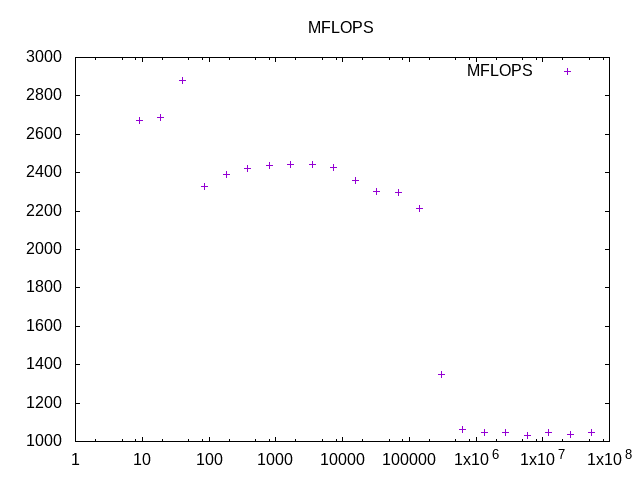
\includegraphics[width=.9\linewidth]{MFLOPS.png}
\end{center}

Above is a graph comparing array length to MFLOPS. Clearly there is a precipitous drop off in performance as N gets large. This is likely due to the increased number of cache misses 
\end{document}